\documentclass[crop, tikz]{standalone}
\usepackage{tikz}
\usepackage{braids}

% base-pair bond: colored tips joined by a dotted hydrogen-bond segment
\newcommand{\bond}[3]{
  \draw[very thick, #1] (#3, 0) -- (#3, 0.35);
  \draw[very thick, densely dotted] (#3, 0.35) -- (#3, 0.65);
  \draw[very thick, #2] (#3, 0.65) -- (#3, 1);
}

\begin{document}
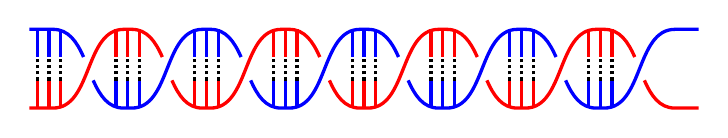
\begin{tikzpicture}
  \foreach \grp in {0, 2, 4, 6} {
    \bond{red}{blue}{\grp + 0.1}
    \bond{red}{blue}{\grp + 0.25}
    \bond{red}{blue}{\grp + 0.4}
  }
  \foreach \grp in {1, 3, 5, 7} {
    \bond{blue}{red}{\grp + 0.1}
    \bond{blue}{red}{\grp + 0.25}
    \bond{blue}{red}{\grp + 0.4}
  }
  \braid[rotate=90,
    style strands={1}{red, very thick},
    style strands={2}{blue, very thick}] (helix) at (0, 0)
    s_1 s_1 s_1 s_1 s_1 s_1 s_1 s_1;
\end{tikzpicture}
\end{document}
